\chapter{提案法}
\section{想定システム}
本稿では,図\ref{fig:soutei}に示すような複数ユーザが利用するリンクに対してボトルネックリンクが存在する環境を仮定する.
\begin{figure}[hh]
\centering
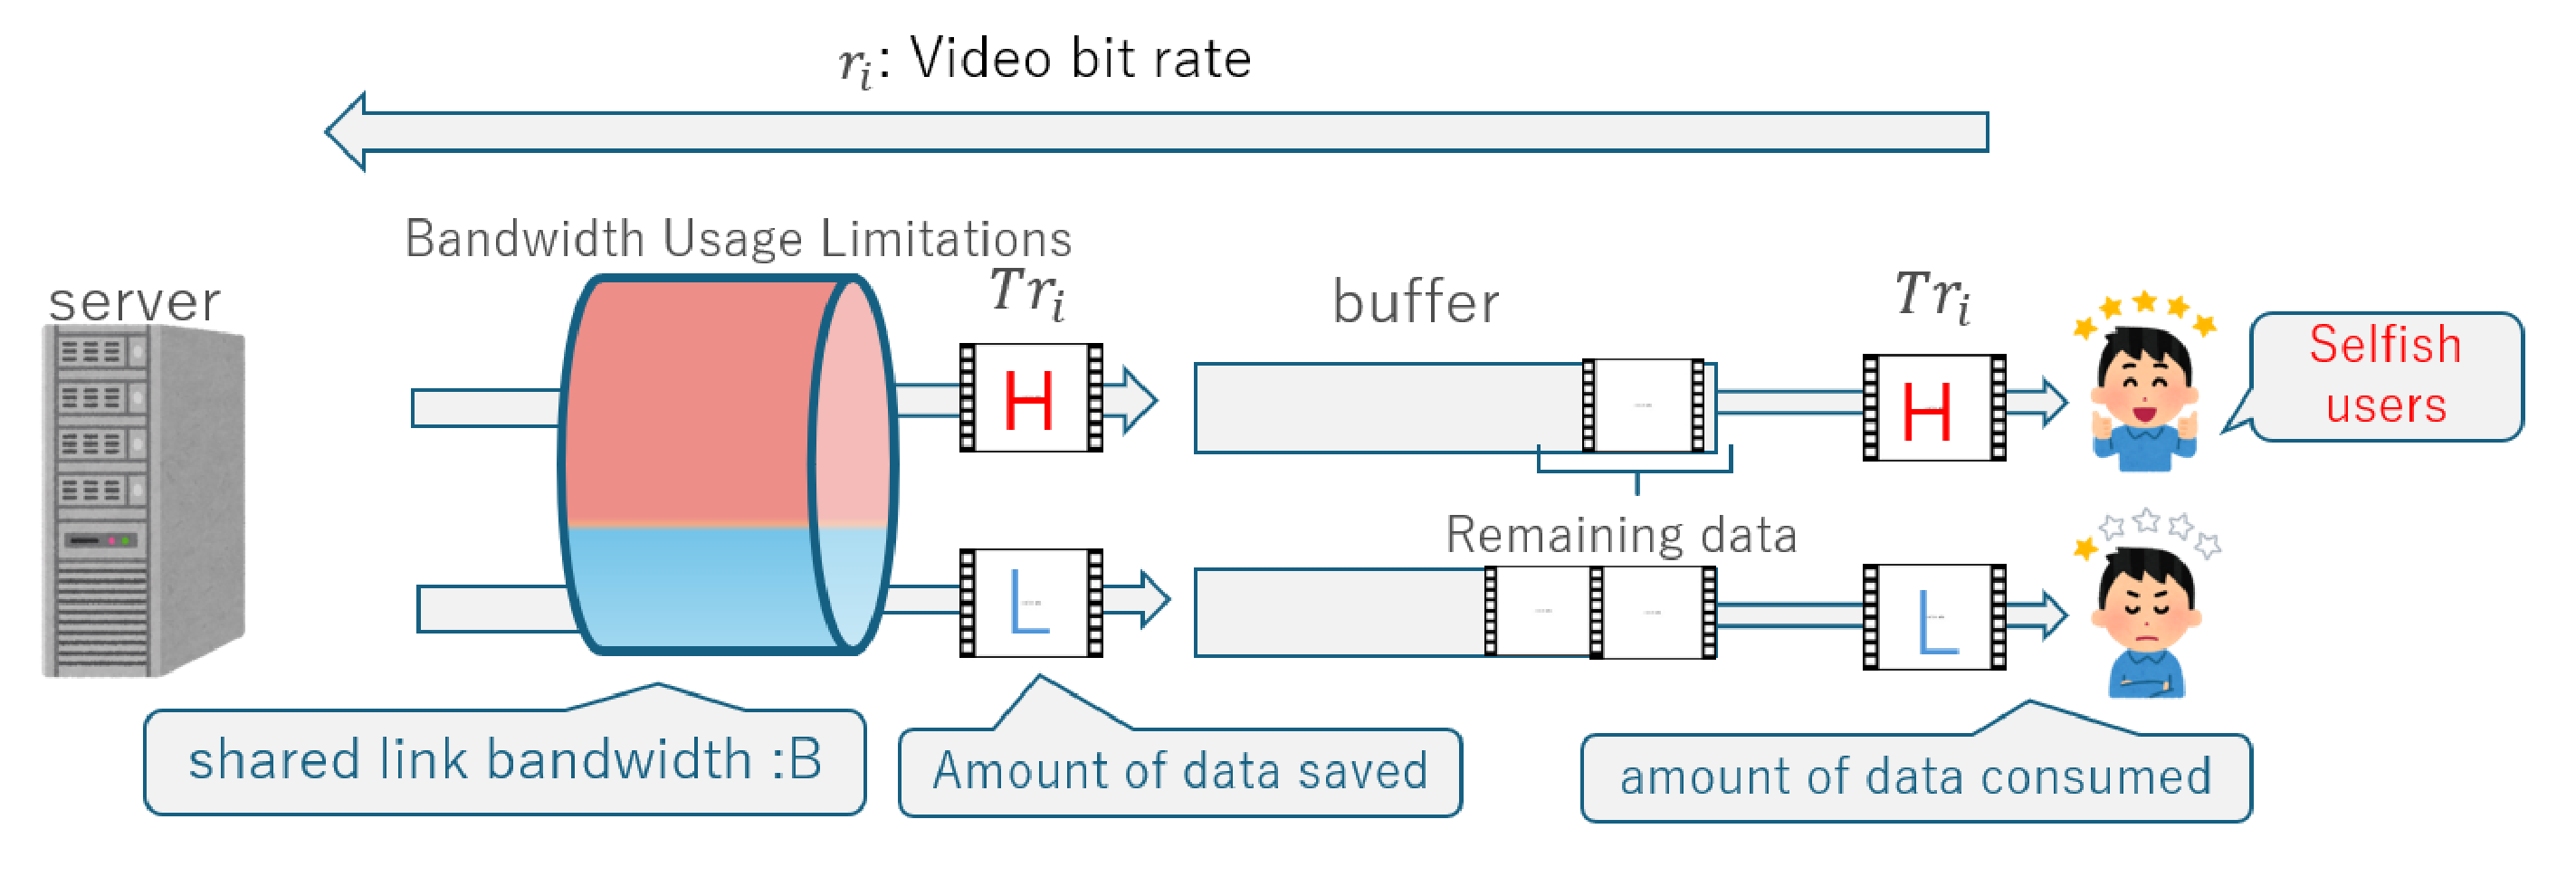
\includegraphics[scale=0.3]{sisutemu.eps}
\bicaption{想定システム}%
            {Assumed system}
\label{fig:soutei}
\end{figure}
ボトルネックリンクの環境では,使用可能帯域幅が狭まっており,ユーザの要求ビデオビットレートが共有しているその他ユーザの使用するはずの帯域に大きく影響し,使用可能帯域を狭め,影響を受けたユーザが動画の再生停止に陥りやすくなる問題がある.そこで,本研究では各ユーザの要求ビデオビットレートによるその他ユーザの使用帯域への影響を考慮するために,ゲーム理論を用いてこの問題をモデル化する.

\section{提案法}
処理の流れは,図\ref{fig:syori}に示す\cite{motomoto}.
まず初めに,ユーザはサーバにセグメント単位で,動画のビデオビットレートを要求する.次に,サーバ側で要求されたビデオビットレートと利用帯域幅の大きさを考慮して,提案利得関数を用いてナッシュ均衡点となる最適ビデオビットレートを導出する.その後,サーバ側で決定したビデオビットレートのデータをユーザ側に送信する流れである.本研究では,この流れの利得関数の改善に着目して提案を行う.

\begin{figure}[hh]
\centering
\includegraphics[scale=0.23]{syori.eps}
\bicaption{処理の流れ}%
            {Processing flow}
    \label{fig:syori}
\end{figure}

ゲーム理論では,相手のとる戦略を考慮しながら自身の利益が最大となる戦略をとる数理モデルを解析する.ストリーミングにおける帯域分配問題において,ユーザ同士は意思疎通を図り協力することができないため,そのようなユーザが協力できない状況をモデル化する,非協力ゲームを用いる.非協力ゲーム理論を用いることで,複数の利己的なユーザが,帯域幅を争う状況ををモデル化し,複数ユーザ間の相互影響における動画の再生停止に陥りやすくなる問題を解析する.

本研究では,ユーザ$i$の最適ビデオビットレート$r_i^*$を決定するため,非協力ゲームを用いて,各ユーザが自身の戦略であるビデオビットレートを変更してもこれ以上利益が増えない状態である最適応答となる戦略レートの組み合わせ(以降,ナッシュ均衡点と呼ぶ)を求める.本研究では,$N=$\{$1,2,3,\dots,n$\},ユーザの選択可能レート$r_i$,ユーザ$i$の利得関数を$f_i$とすると,$G=\left(N,{r_i}_{(i\in N)},{f_i}_{(i\in N)}\right)$とモデル化することができる.
本研究では,ナッシュ均衡点を利得関数によって決定する.

\section{ビデオビットレート制御法}

%%下の説明をどこに入れるか
本研究では,既存研究\cite{kison}と\cite{motomoto}で用いられている利得関数を基に,関数の一部を変更したものであるため,まずは既存研究での利得関数\cite{kison}\cite{motomoto}について説明を行う.

以下に非協力ゲームレート制御法\cite{kison}の$f_i$を示す.
\begin{equation}
 f_{i}=\underbrace{q_{i}(r_{i,k})}_{(\rm{A})}+\underbrace{\mu\Delta{b^{\rm{est}}_{i,k}}(r_{i,k},\mathbf{r}_{-i,k})}_{(\rm{B})}+\underbrace{\gamma_i{R}_{\rm{f}}(r_{i,k})}_{(\rm{C})}.
 \label{eq:f1}
\end{equation}
以下に,より詳細な式を示す.
\begin{equation}
\begin{split}
  f_i(r_k) = &\ \underbrace{\alpha_{\text{ct}} \log(1 + |\beta_{\text{ct}}| r_{i,k})}_{(\rm{A})} \\
  &+ \underbrace{\mu \frac{2 e^{p(b_{i,k-1} - b_s)}}{1 + e^{p(b_{i,k-1} - b_s)}}\left(  T r_{i,k} \right) - \mu \omega  \left( T \frac{r_{i,k}^2 + r_{i,k} \sum_{l \neq i} r_{l,k}}{B_W} \right)}_{(\rm{B})} \\
  &+ \underbrace{\gamma_i \left( -m(r_{i,k} - r_{i,k-1} + r^{(J)})^2 - 2m(r_{i,k} - r_{i,k-1}) \right)}_{(\rm{C})}
  \label{eq:syousai}
\end{split}
\end{equation}



非協力ゲームレート制御法\cite{kison}では,式\eqref{eq:f1}基い\eqref{eq:syousai}を用いて最適レートを導出していた.
(A)項はビデオビットレートのみから得られる嬉しさを表す単調増加の関数である.
(B)項はバッファの変動量を用いてユーザのビデオビットレートを制御する関数である.
(C)項は前のセグメントで決定したビデオビットレートとの変動差を抑える関数である.
ここで,大きくビデオビットレートの制御を行っているのは,(B)項であった.
次に,(B)項を説明する.以下に,(B)項の基本構造を示す.
\begin{equation}
 f_{buffer}=Tr_{i,k}-Tr_{i,k}\underbrace{(\frac{\sum^N_{i=1}r_{i,k}}{B})}_{\rm{(D)}}
 \label{eq:f_{buffer}}
\end{equation}

式\eqref{eq:f_{buffer}}は,あるセグメントにおけるバッファの変動量を表している.
$T$はセグメント長[s],$r_i$はビデオビットレート[Mbps],$B$はリンクの全帯域幅[Mbps]を表す.
1項目はバッファにたまるのデータ量を表し,2項目は1項目のデータがバッファに溜まりきるまでの時間でバッファから消費されるデータ量を表す.

ここで,式\eqref{eq:f_{buffer}}の(D)は要求に対するペナルティを与える補正項を表している.全帯域に対して全ユーザの合計要求ビデオビットレートの方が大きいと,要求ビデオビットレートのデータがバッファにダウンロードされるまでに時間がかかり,その間,よりバッファからデータが消費される.バッファにデータがたまっていない状態をバッファ枯渇と言い,再生できる動画データがないため,動画の再生停止が起きる.

この補正項では,ユーザ毎の要求ビデオビットレートの大きさに応じてペナルティを与えていない.そのため,帯域を狭めている大きいビデオビットレートを要求した利己的なユーザも,小さいビデオビットレートを要求したユーザも同じペナルティが与えられ,制限がかけられる.それは,以下の表\ref{tb:ritoku1}を見れば明らかである.表\ref{tb:ritoku1}では,セグメント長が1sで二人のユーザが4Mbpsの帯域を争ったときの二人の利得を示す.二人のユーザは$1\sim6$Mbpsのビットレートを要求することができ,各レートを要求したときの利得を式\eqref{eq:f_{buffer}}を用いて計算している.表内の値は,(ユーザ1の利得,ユーザ2の利得)である.
%%以下101行目の1文修正箇所

\begin{table}[h]
    \centering
    \bicaption{非協力ゲームレート制御法\cite{motomoto}の利得表}
            {Non-cooperative game rate control method\cite{motomoto} gain table}
    \scalebox{0.7}{
    \begin{tabular}{|c|c|c|c|c|c|c|}
        \hline
        \diagbox{user1}{user2} & 1 & 2 & 3 & 4 & 5 & 6 \\ \hline
        1 & (0.5, 0.5) & (0.25, 0.5) & (0.0, 0.0) & (-0.25, -1.0) & (-0.5, -2.5) & (-0.75, -4.5) \\ \hline
        2 & (0.5, 0.25) & (0.0, 0.0) & (-0.5, -0.75) & (-1.0, -2.0) & (-1.5, -3.75) & (-2.0, -6.0) \\ \hline
        3 & (0.0, 0.0) & (-0.75, -0.5) & (-1.5, -1.0) & (-2.25, -3.0) & (-3.0, -5.0) & (-3.75, -7.5) \\ \hline
        4 & (-1.0, -0.25) & (-2.0, -1.0) & (-3.0, -2.25) & (-4.0, -4.0) & (-5.0, -6.25) & (-6.0, -9.0) \\ \hline
        5 & (-2.5, -0.5) & (-3.75, -1.5) & (-5.0, -3.0) & (-6.25, -5.0) & (-7.5, -7.5) & (-8.75, -10.5) \\ \hline
        6 & (-4.5, -0.75) & (-6.0, -2.0) & (-7.5, -3.75) & (-9.0, -6.0) & (-10.5, -8.75) & (-12.0, -12.0) \\ \hline
    \end{tabular}
    }
    \label{tb:ritoku1}
\end{table}

縦軸のユーザ1のみが6Mbps,横軸のユーザ2が1Mbpsをとった時のそれぞれの利得は,利己的な要求をしているユーザ1のみだけでなく,低ビデオビットレートを要求しているユーザ2にもペナルティがかかり,ユーザ2の利得も同時に下がっている.

そのため,本研究ではユーザの要求ビデオビットレートと他ユーザへの影響度合いを考慮したペナルティ関数に変更する.


\section{提案利得関数}
次に提案する利得関数について説明する.以下にその式を示す.
\begin{equation}
    f_{\mathrm{buffer}}(i) = Tr_{i,k} - Tr_{i,k}\underbrace{\left(\frac{r_{i,k}}{B\left(1-\frac{r_{i,k}}{\sum^N_{j=1}r_{j,k}}\right)}\right)}_{\rm{E}}
    \label{eq:f_buffi}
\end{equation}

本利得関数では,ユーザ$i$のビデオビットレート要求が他ユーザの使用帯域に与える影響を評価する補正項を導入している.次に,Eの補正項の具体的な式を示す.
\begin{equation}
    f_{\mathrm{penalty}}=\frac{r_{i,k}}{B\left(1-\frac{r_{i,k}}{\sum^N_{j=1}r_{j,k}}\right)}
    \label{eq:f_{penalty}}
\end{equation}

この補正項は,ユーザ$i$の使用可能帯域の割合を
\begin{equation}
    B_{i}=B\frac{r_{i,k}}{\sum^N_{j=1}r_{j,k}}
    \label{eq:B_{i}}
\end{equation}
を用いて算出し,それに基づいて他ユーザの使用可能帯域への影響を評価するものである\cite{johari}.具体的には,全帯域$B$からユーザ$i$の使用可能帯域を引いた値が,残りの他ユーザの使用可能帯域を表している.この補正項\ref{eq:f_{penalty}}により,ユーザ$i$の利得は,自身のビデオビットレート要求が他ユーザの使用可能帯域をどの程度圧迫するかに応じて調整される.

また,$r_i$のみを増加させた場合,式\ref{eq:B_{i}}の値が増加し,補正項の分母が減少するため,ユーザ$i$のペナルティが増加する.一方,他ユーザも同時にビデオビットレートを増加させると,全帯域$B$が要求比率に基づき分配され,結果として全ユーザに均等なペナルティが与えられる.つまり,ユーザ$i$のみが利己的な要求を行った場合,そのペナルティが最も大きくなる.